% See exam.cls and examdoc.tex for the license information
\documentclass[12pt, answers]{exam}

\usepackage{amssymb}
\usepackage{makeidx}
\usepackage{amsmath}
\usepackage{graphicx}
\usepackage{caption}
\usepackage{tabulary}
\usepackage{color}
\usepackage{multicol}
\usepackage{multirow}
\usepackage{enumerate}
\usepackage{float}
\usepackage{colortbl}
\usepackage[table,xcdraw]{xcolor}

\usepackage{array}
\newcolumntype{C}[1]{>{\centering\let\newline\\\arraybackslash\hspace{0pt}}m{#1}}

\addpoints

% In case we're not using hyperref.sty:
\providecommand{\texorpdfstring}[2]{#1}
% The following can be used in \section commands
% without generating pdf warnings:
\newcommand{\bs}{\texorpdfstring{\char`\\}{}}

\makeindex

\newcommand{\indc}[1]{\index{#1@\texttt{\char`\\#1}}}
\newcommand{\indcsub}[2]{\index{#1@\texttt{\char`\\#1}!#2}}
\newcommand{\indcstart}[1]{\index{#1@\texttt{\char`\\#1}|(}}
\newcommand{\indcstop}[1]{\index{#1@\texttt{\char`\\#1}|)}}

\newcommand{\indt}[1]{\index{#1@\texttt{#1}}}
\newcommand{\indtsub}[2]{\index{#1@\texttt{#1}!#2}}
\newcommand{\indtstart}[1]{\index{#1@\texttt{#1}|(}}
\newcommand{\indtstop}[1]{\index{#1@\texttt{#1}|)}}

\extraheadheight{-.4in}

\pagestyle{headandfoot}
%\extraheadheight{.2 in}
\firstpageheader{}{}{}
\runningheader{}{}{}
\firstpagefooter{INF281}{Exercise 10}{Page \thepage\ of \numpages}
\firstpagefootrule
\runningfooter{INF281}{Exercise 10}{Page \thepage\ of \numpages}
\runningfootrule

%---------------------------------------------------------------------

\shadedsolutions
\noprintanswers
\definecolor{SolutionColor}{rgb}{0.8,0.9,1}

\begin{document}

\section*{INF281 Exercise 10}

%---------------------------------------------------------------------
\begin{questions}

%%% Question 1
\question \textbf{HMM probabilities}

An HMM (hidden Markov model) is a probabilistic graphical model with three types of probabilities.

\noindent
Transition probabilities:
\begin{table}[H]
\centering
\begin{tabular}{|c|c|c|}
\hline
     & $\mathrm{L_t}$  & $\mathrm{H_t}$  \\ \hline
$\mathrm{L_{t-1}}$ & 0.2 & 0.8 \\ \hline
$\mathrm{H_{t-1}}$ & 0.4 & 0.6 \\ \hline
\end{tabular}
\end{table}

\noindent
Emission probabilities:
\begin{table}[H]
\centering
\begin{tabular}{|c|c|c|}
\hline
     & L  & H  \\ \hline
Sunny & 0.5 & 0.7 \\ \hline
Rain & 0.5 & 0.3 \\ \hline
\end{tabular}
\end{table}

\noindent
Initial transition probabilities:
\begin{center}
(L, H) = (0.3, 0.7)
\end{center}

\vspace{0.1 in}

\begin{parts}

%% (a)
  \part Add the transition and emission probabilities to the graph.
\begin{figure}[H]
      \centering
      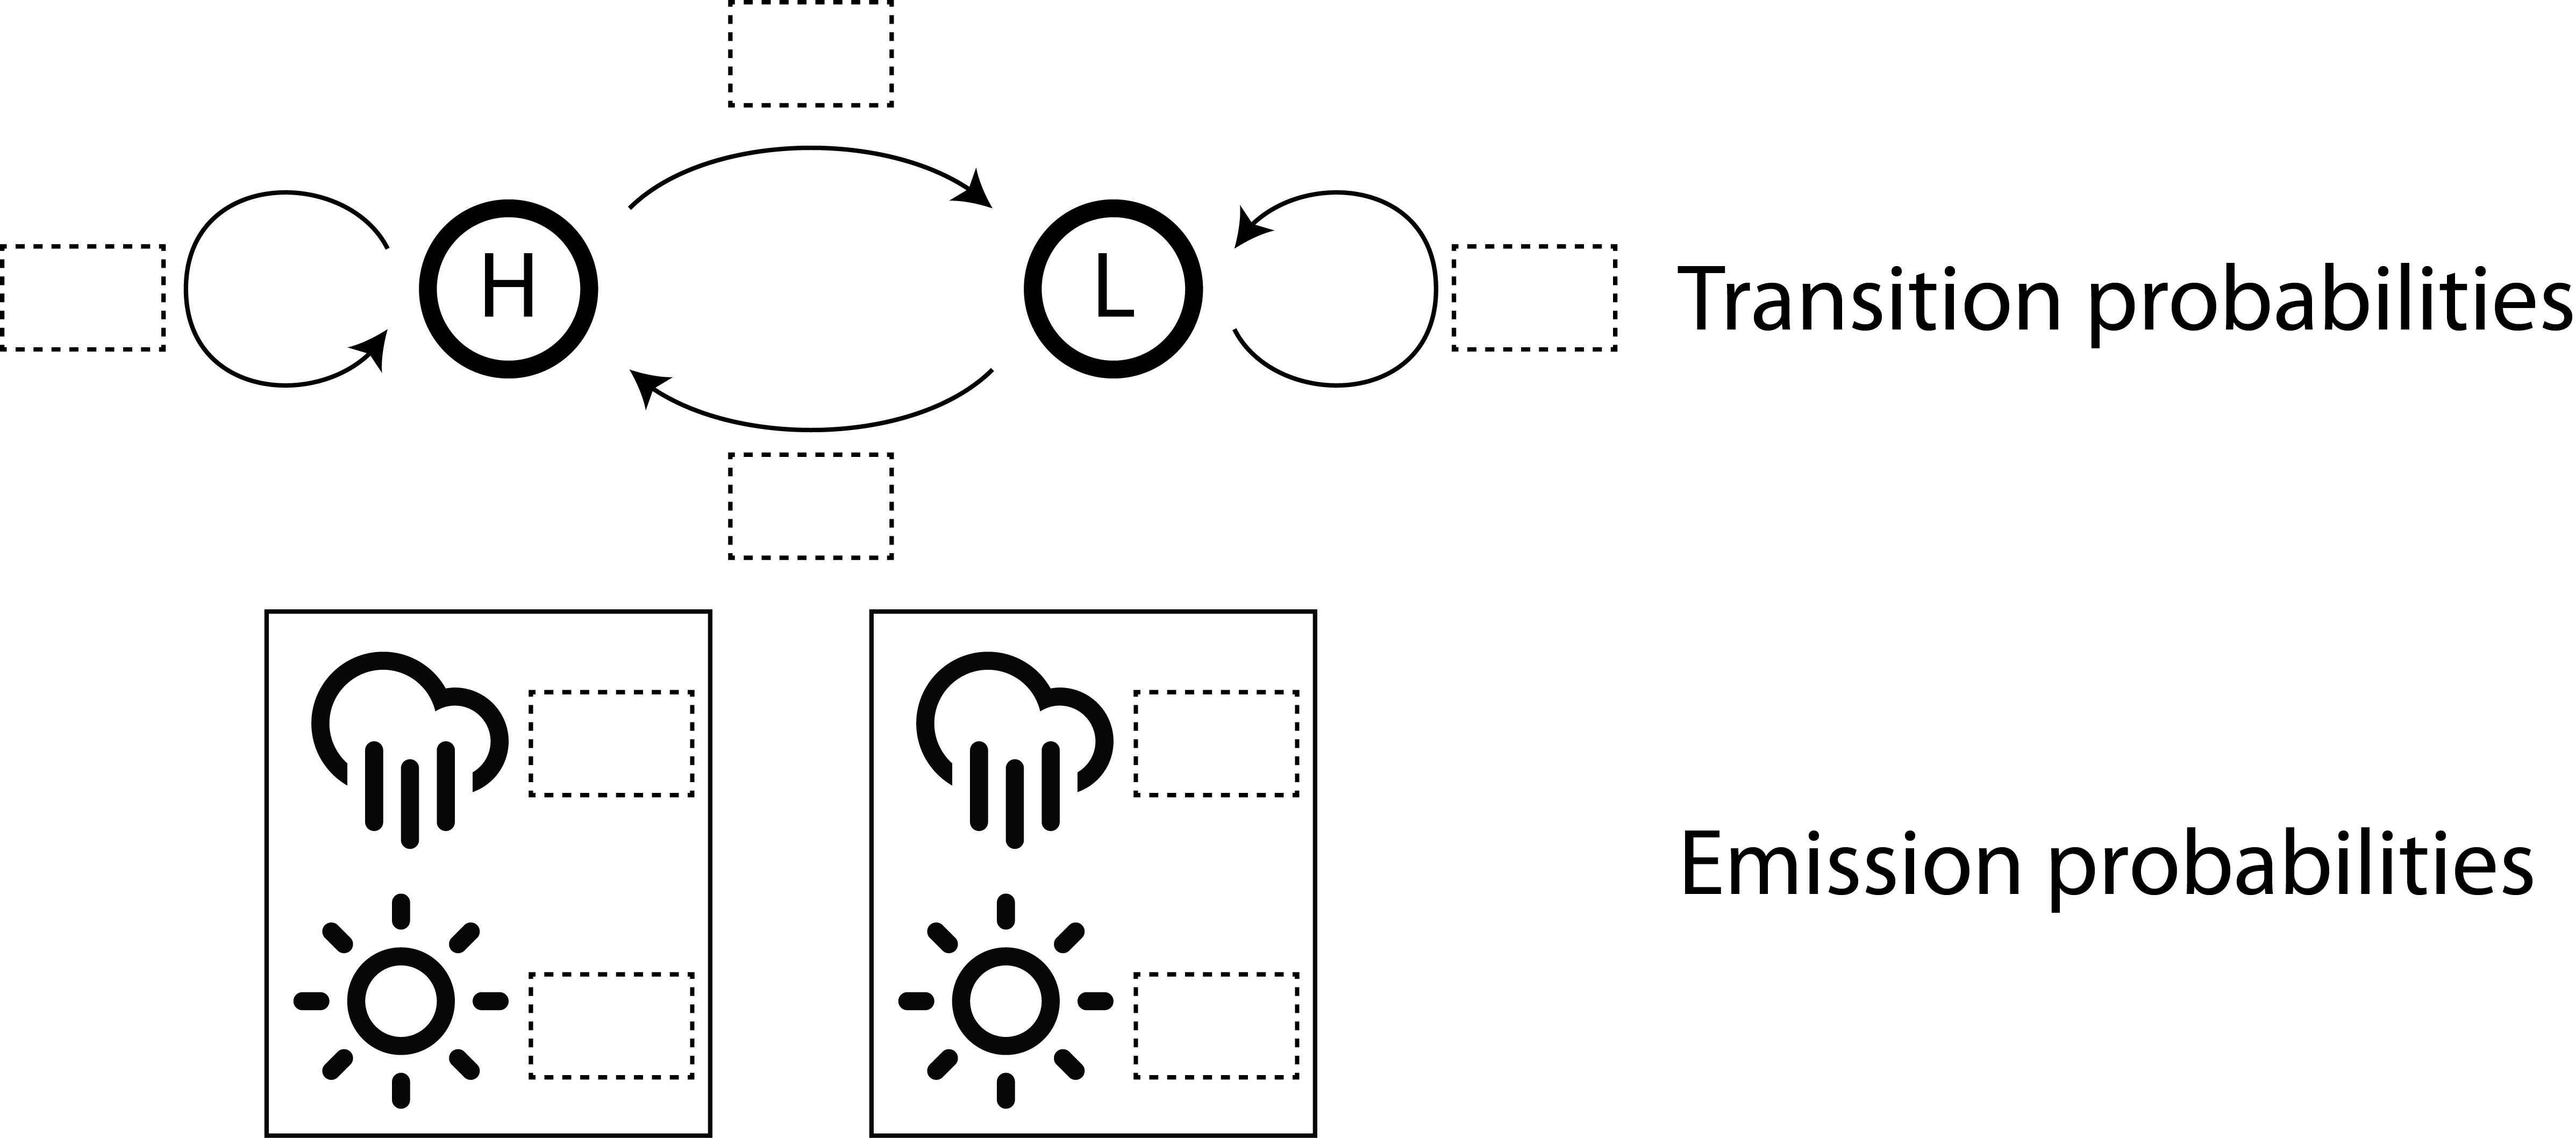
\includegraphics[width=0.6 \textwidth]{fig13/hmm_probabilities.png}
\end{figure}

%% (b)
  \part What are the joint probabilities for (Rain, Rain, Sunny) and (H, L, L)?
\begin{solution}[0.35 in]
p(H)p(Rain$\mid$H) $\times$ p(L$\mid$H)p(Rain$\mid$L) $\times$ p(L$\mid$L)p(Sunny$\mid$L) \\
\null \quad  \quad \quad \quad \quad $= 0.7 \times 0.3 \times 0.4 \times 0.5 \times 0.2 \times 0.5 = 0.0042$
\end{solution}

%% (c)
  \part What are the joint probabilities for (Sunny, Rain, Sunny) and (L, H, L)?
\begin{solution}[0.35 in]
p(L)p(Sunny$\mid$L)  $\times$  p(H$\mid$L)p(Rain$\mid$H) $\times$  p(L$\mid$H)p(Sunny$\mid$L) \\
\null \quad  \quad \quad \quad \quad $= 0.3 \times 0.5 \times 0.8 \times 0.3  \times 0.4 \times 0.5 = 0.0072$
\end{solution}

\end{parts}

\newpage

%%% Question 2
\question \textbf{HMM profile}

A path of an HMM profile represents an alignment between an input sequence and the profile.

\vspace{0.1 in}

\begin{parts}

%% (a)
  \part Assume Seq1 = ’q1 q2’ and its path is indicated with solid lines. Draw the alignment of Seq1 and the profile.
\begin{figure}[H]
      \centering
      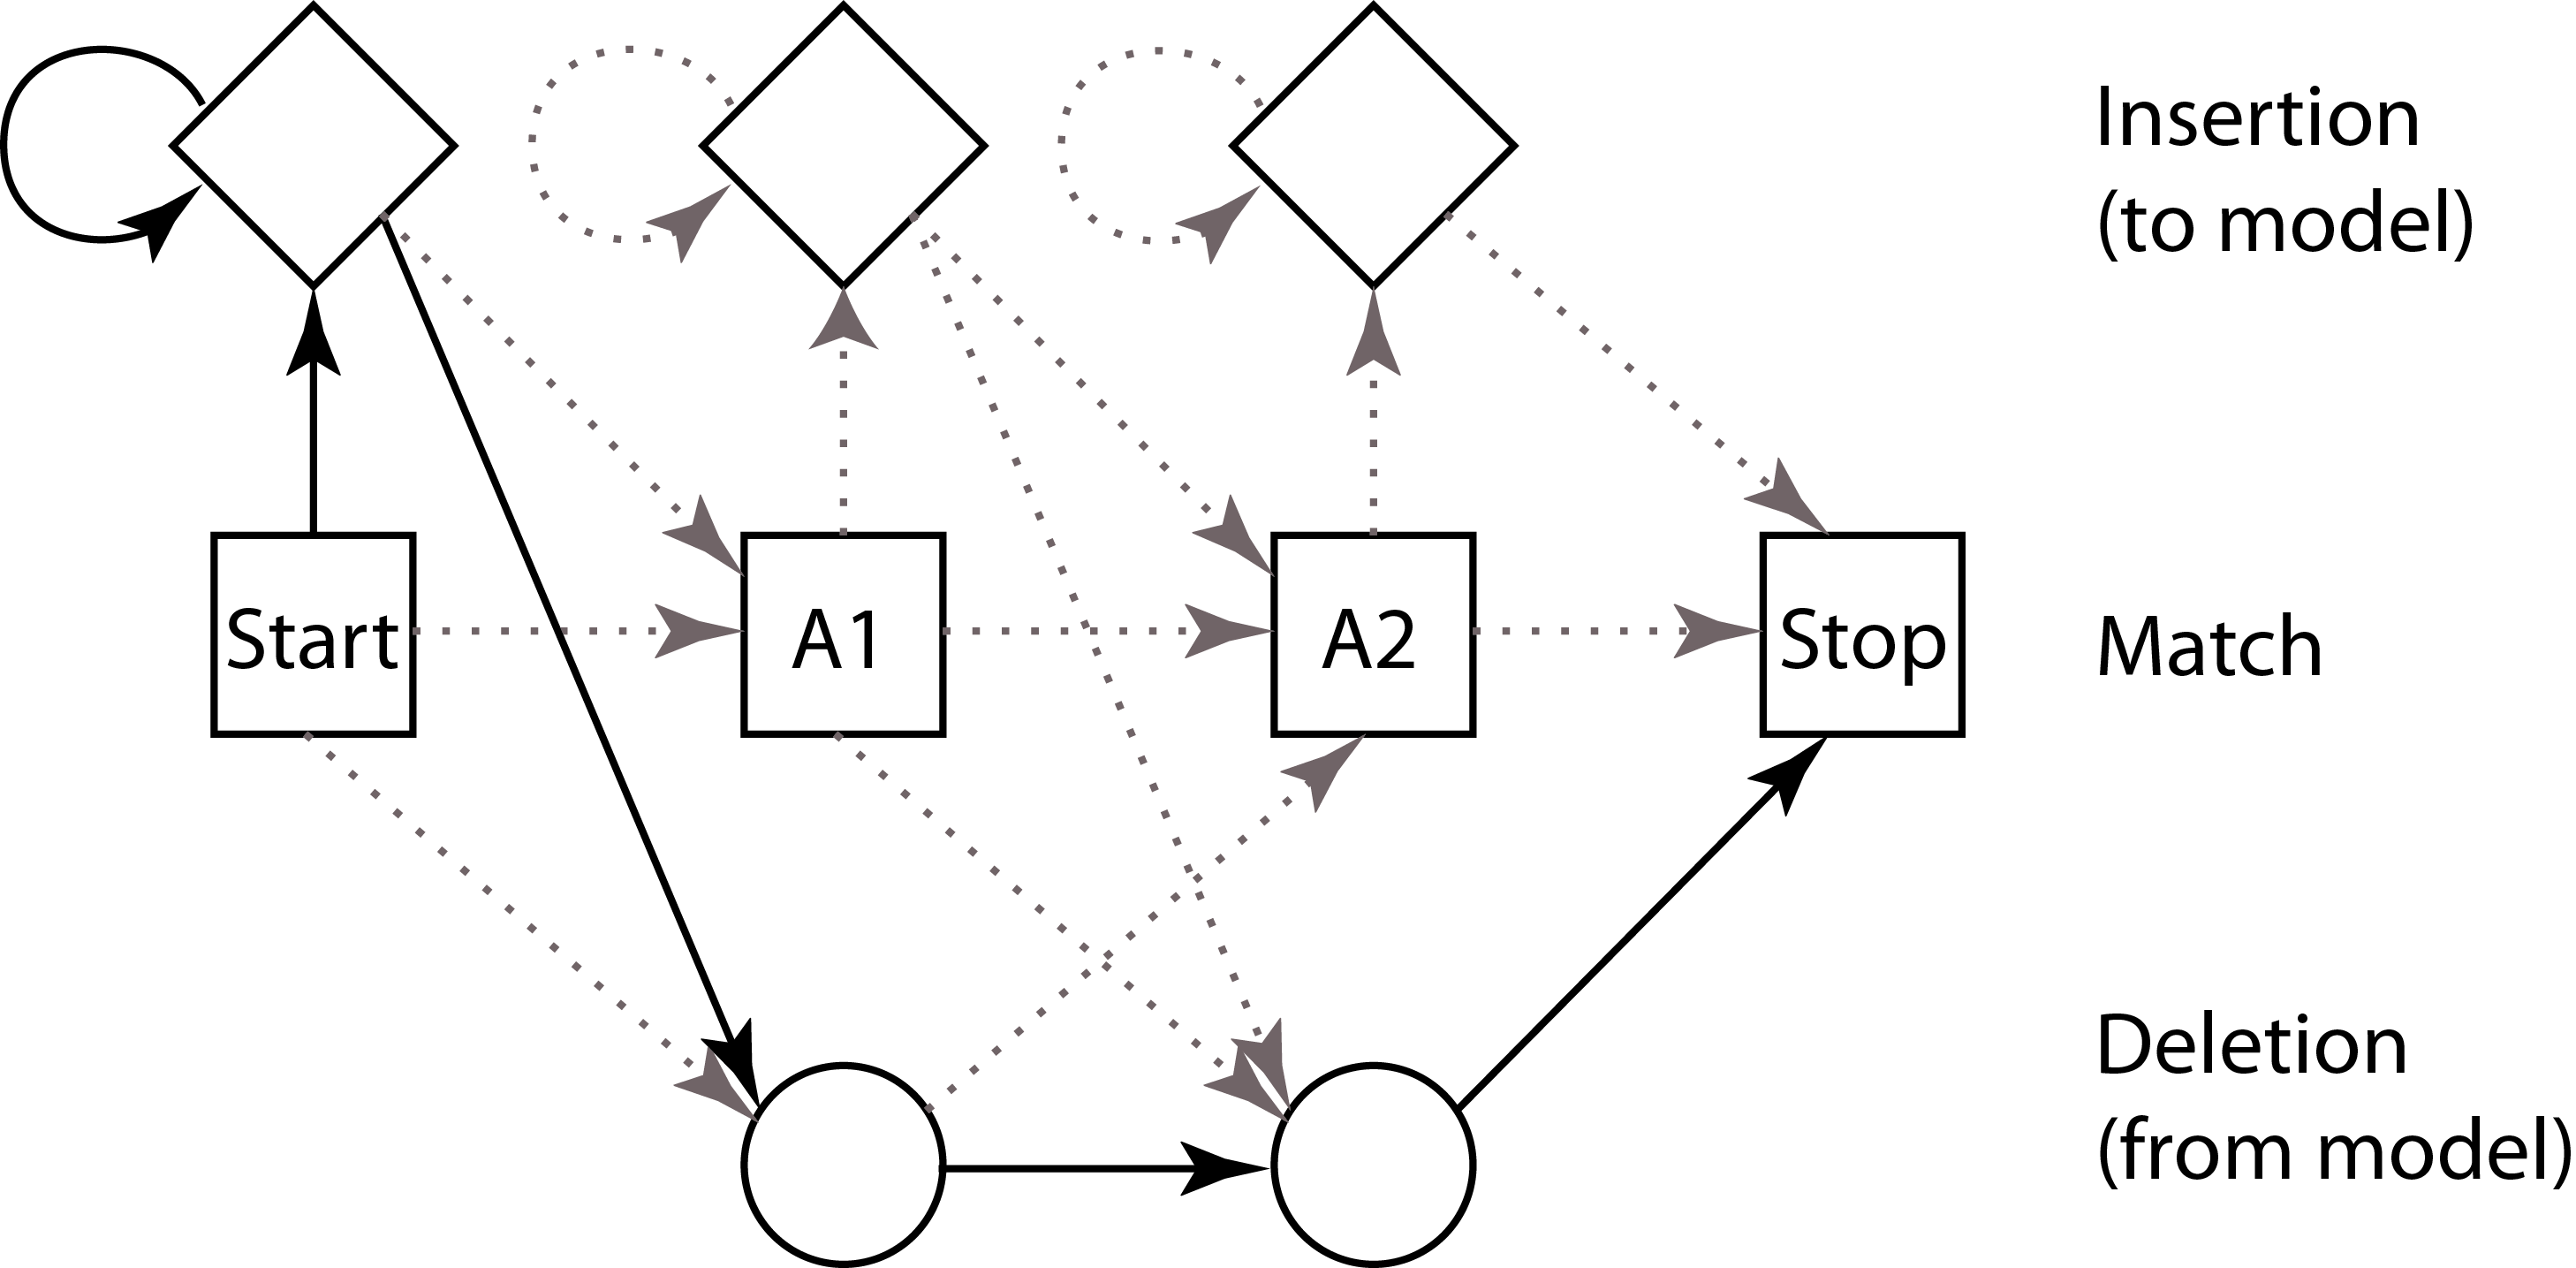
\includegraphics[width=0.6 \textwidth]{fig13/hmm_profile_1.png}
\end{figure}

\begin{solution}[0.7 in]
\begin{verbatim}
   Seq1: q1 q2 -  -
Profile: -  -  A1 A2
\end{verbatim}
\end{solution}

%% (b)
  \part Assume Seq2 = ’q1 q2 q3 q4 q5 q6’ and its path is indicated with solid lines. Draw the alignment of Seq2 and the profile.
\begin{figure}[H]
      \centering
      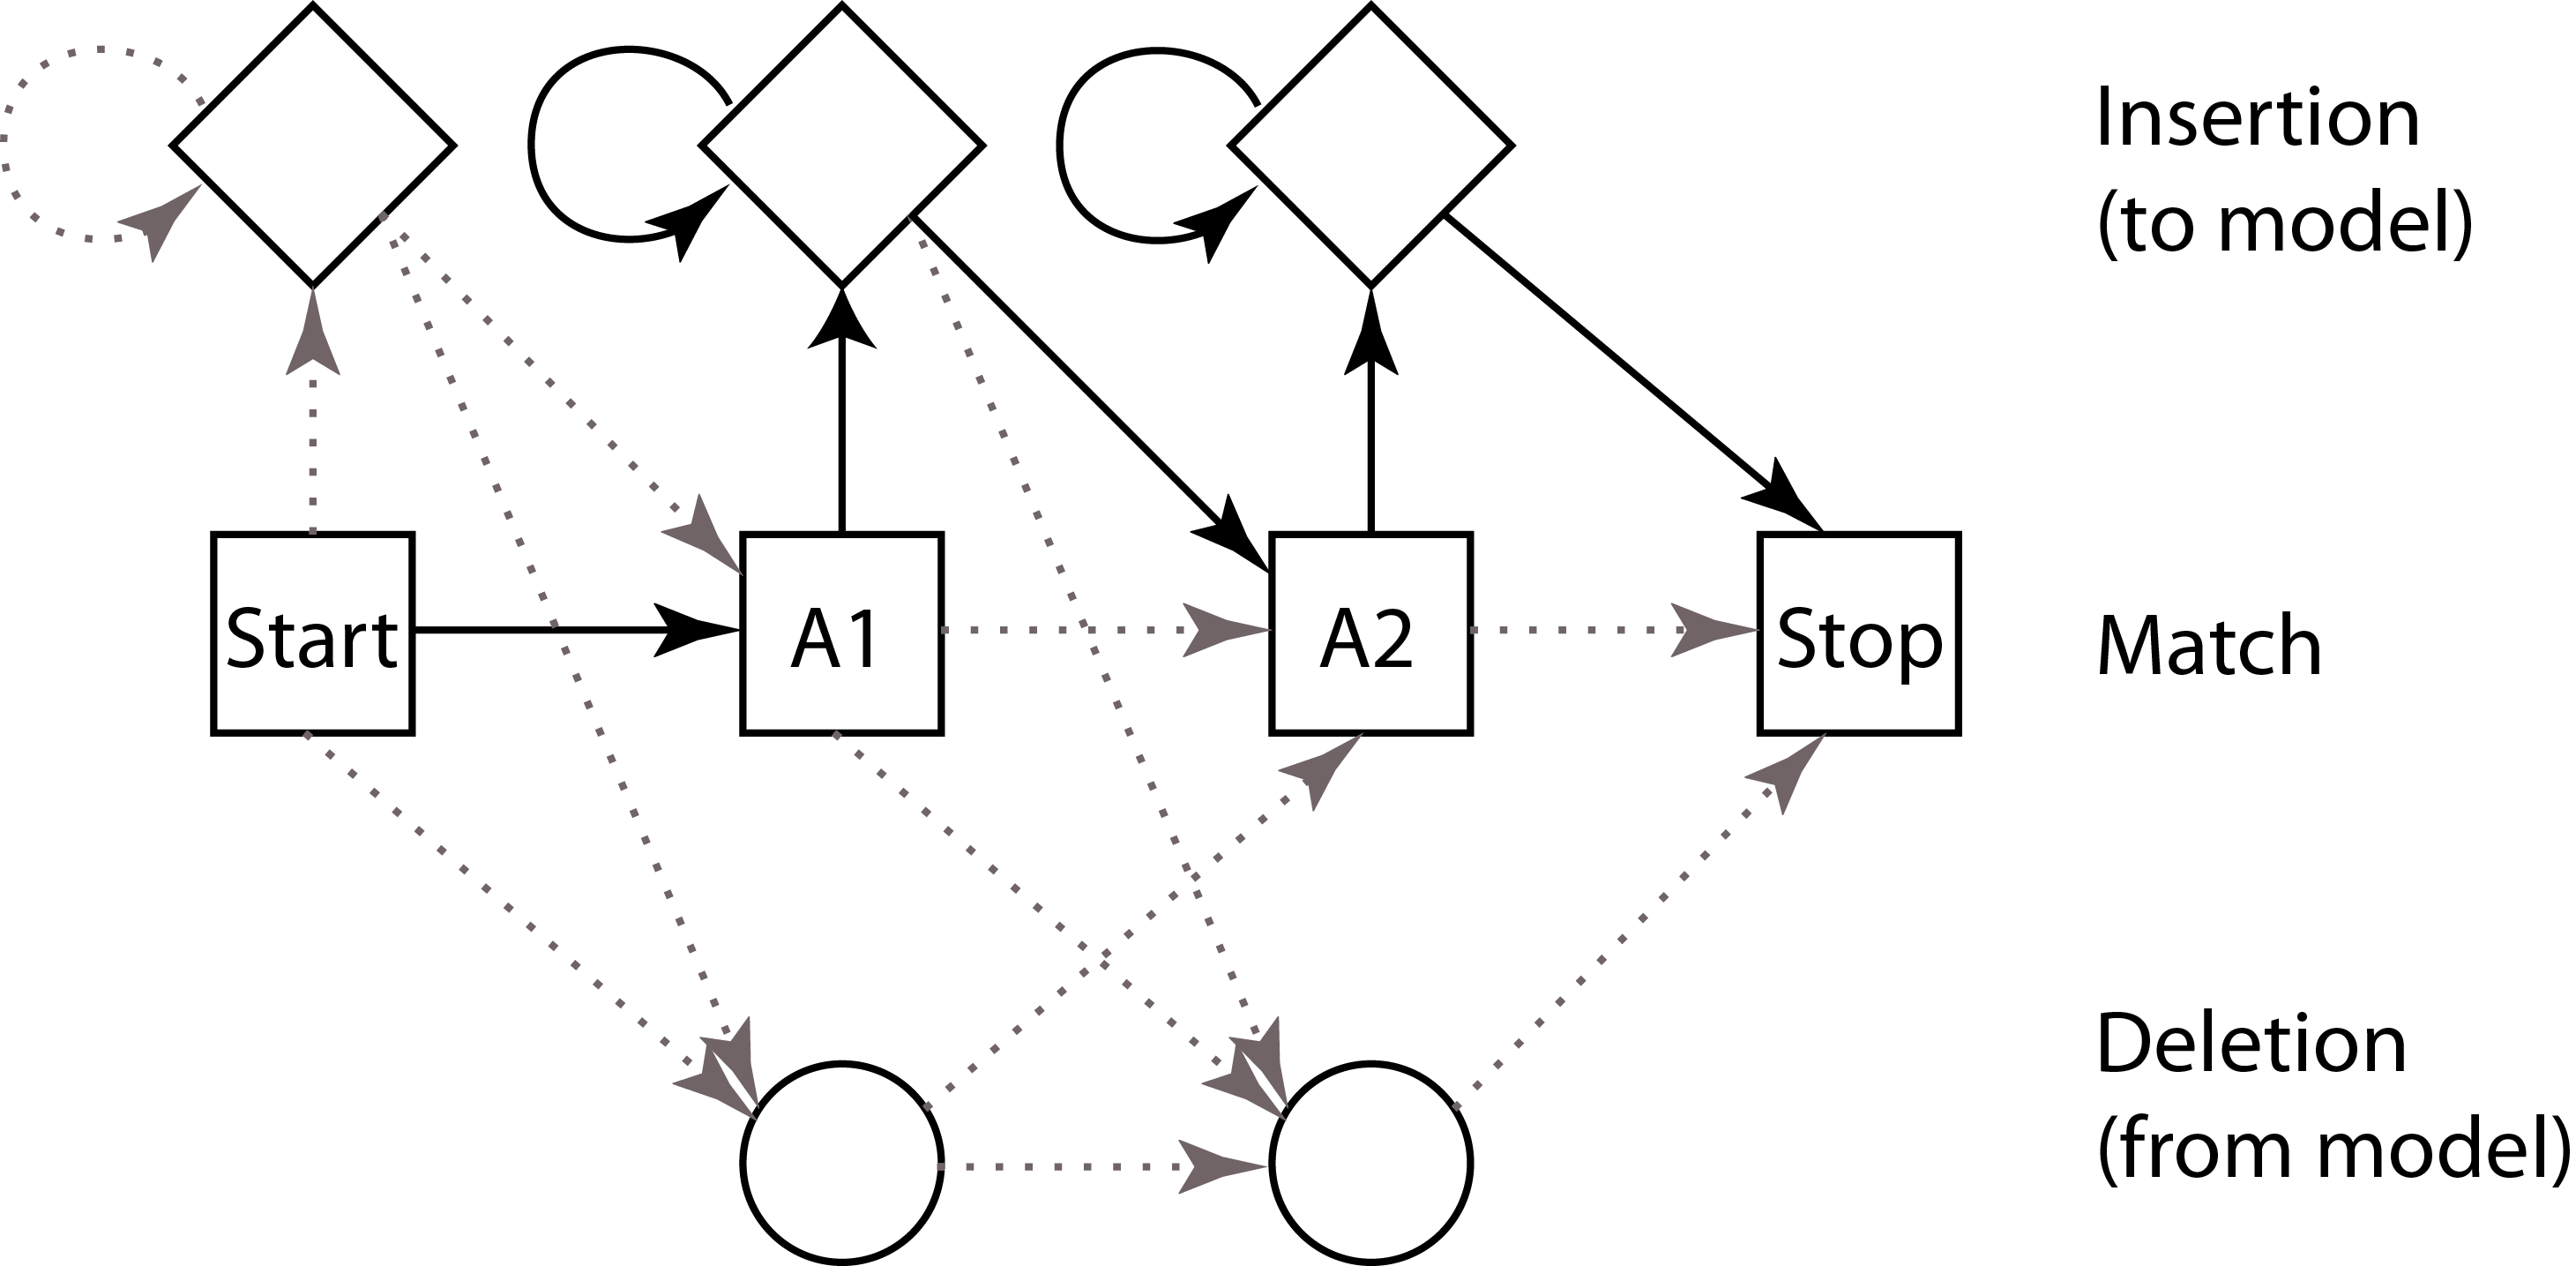
\includegraphics[width=0.6 \textwidth]{fig13/hmm_profile_2.png}
\end{figure}

\begin{solution}[0.7 in]
\begin{verbatim}
   Seq2: q1 q2 q3 q4 q5 q6
Profile: A1 -  -  A2 -  -
\end{verbatim}
\end{solution}

\end{parts}

\newpage

%%% Question 3
\question \textbf{The Viterbi algorithm}

The Viterbi algorithm is a dynamic programming based method to find the optimal path of an HMM with hidden status.

\begin{figure}[H]
      \centering
      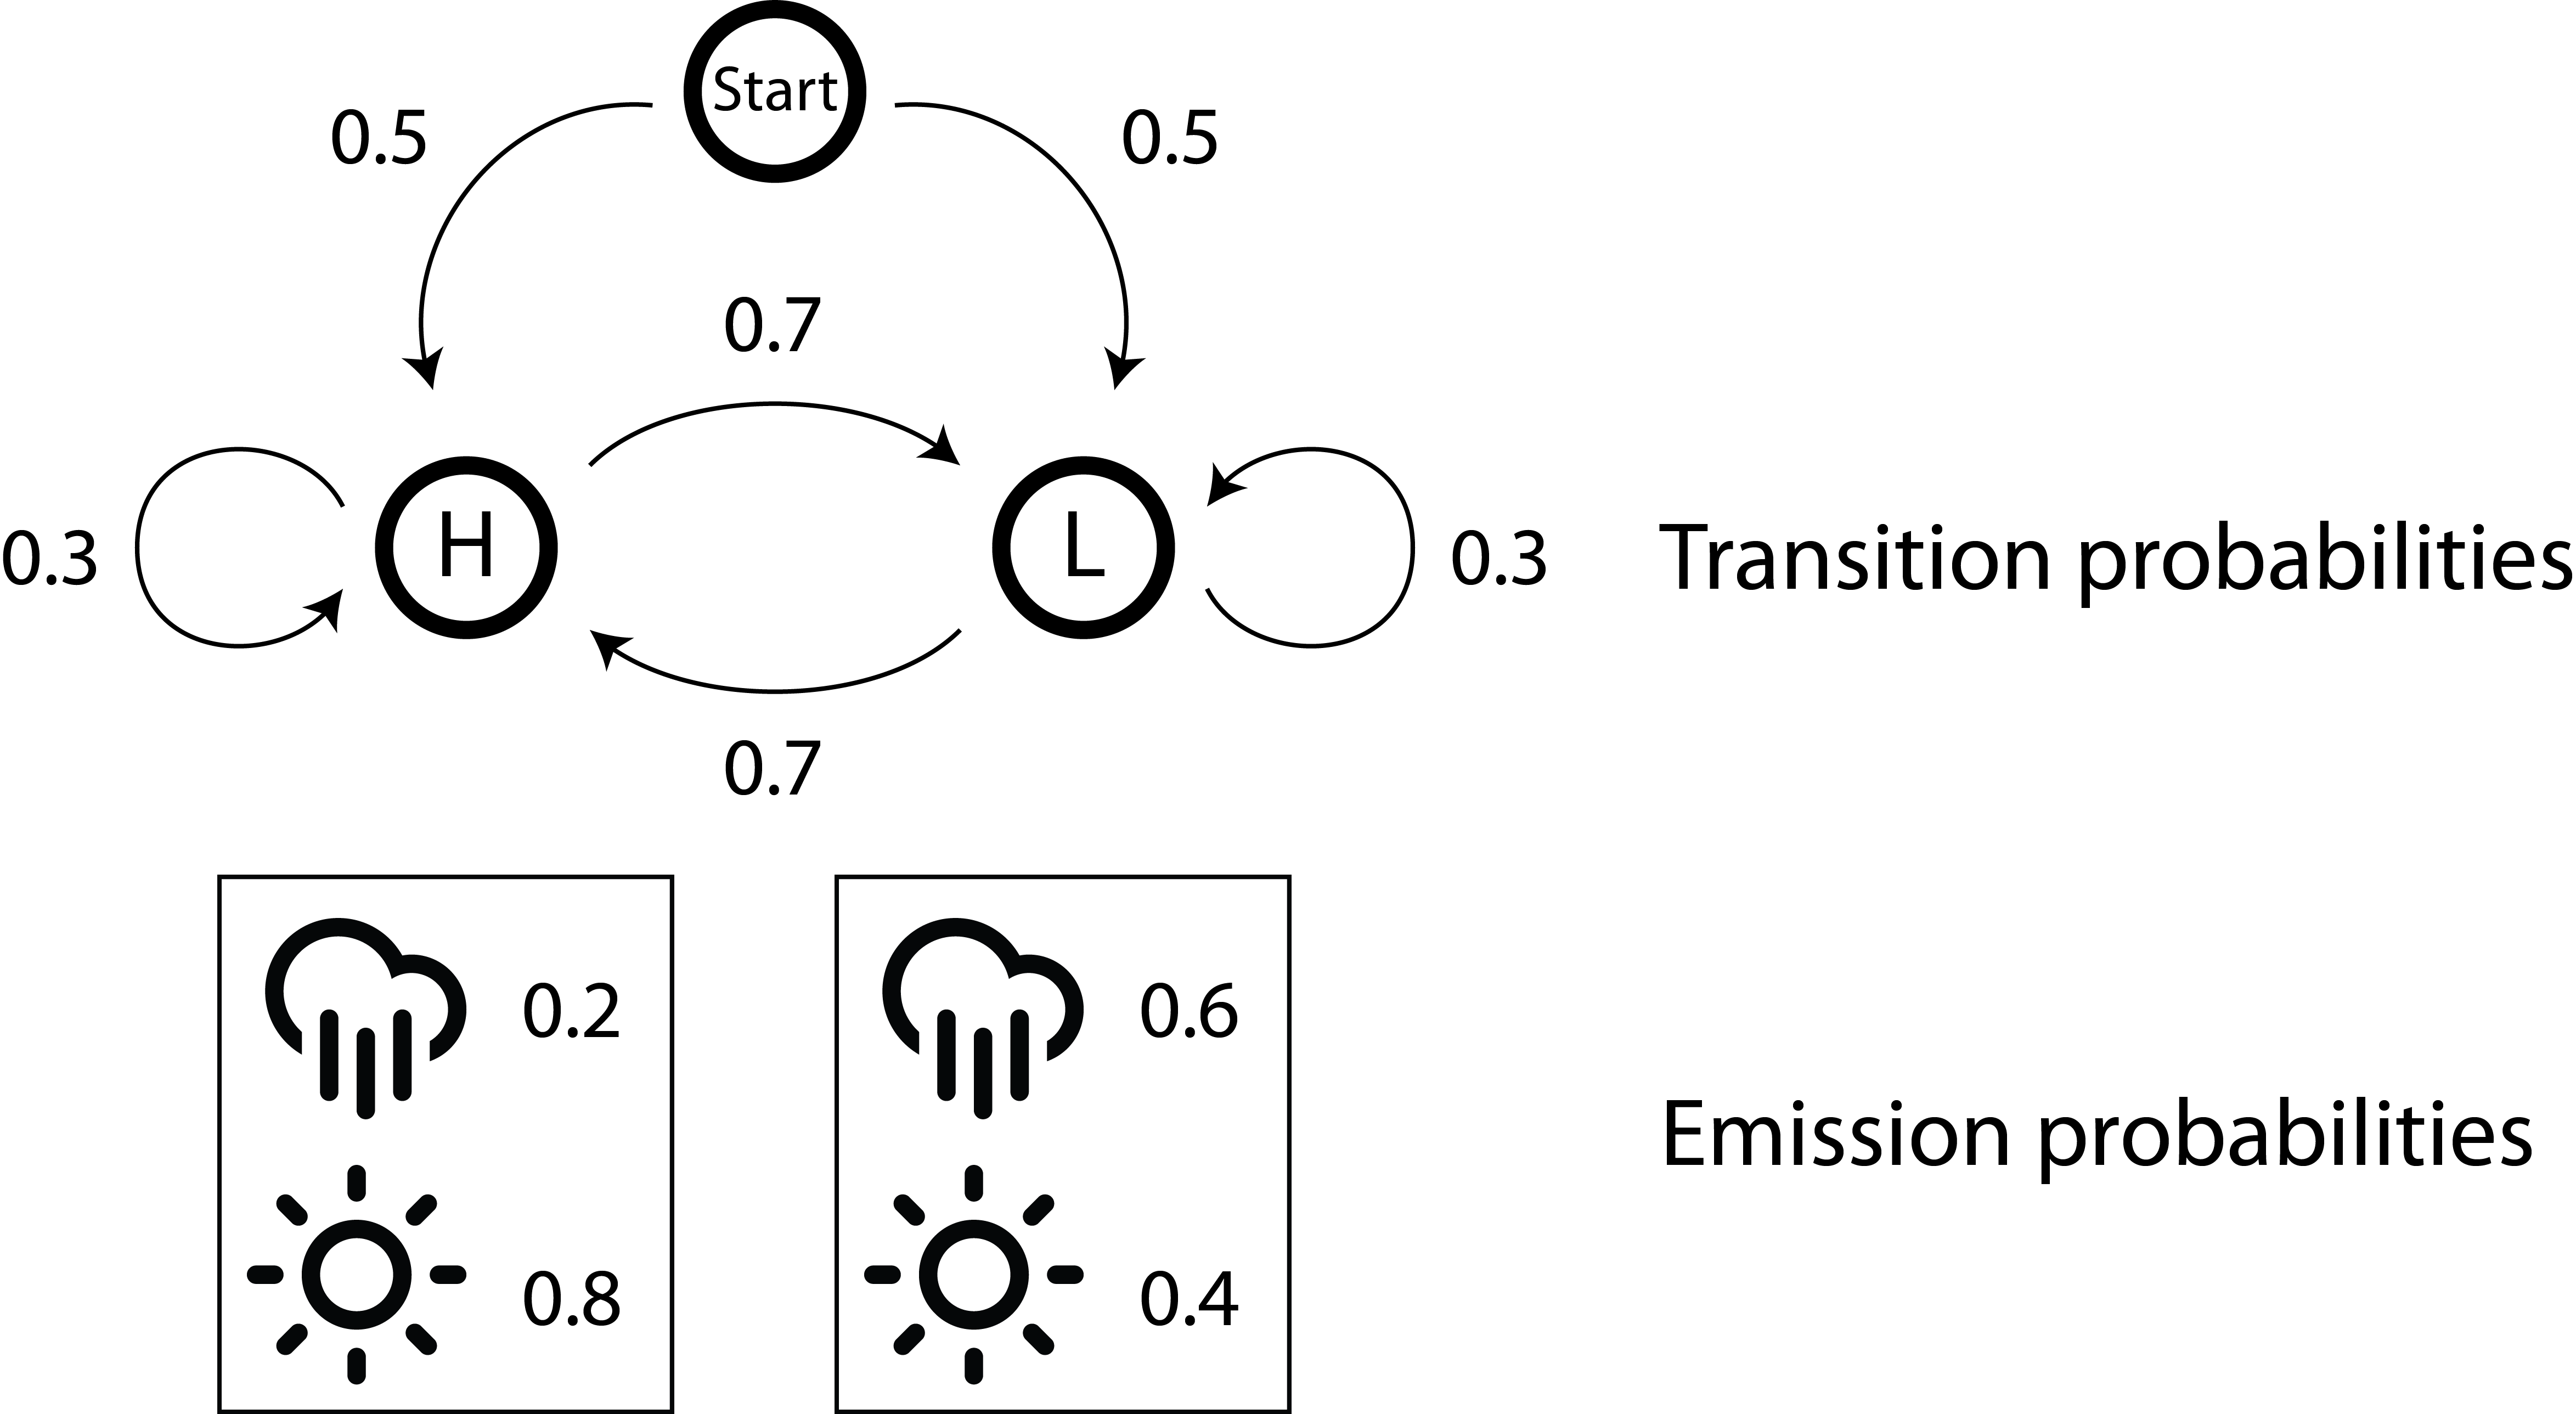
\includegraphics[width=0.6 \textwidth]{fig13/hmm_viterbi.png}
\end{figure}

\vspace{0.1 in}

\begin{parts}

%% (a)
  \part Find the optimal path when observed weather conditions are (Rain, Sunny).
\begin{table}[H]
\centering
\begin{tabular}{|c|c|c|}
\hline
      & H & L \\ \hline
Rain  &  \qquad  \qquad  \qquad  \qquad  \qquad \qquad  \qquad & \qquad  \qquad  \qquad \qquad  \qquad \qquad  \qquad \\ \hline
Sunny &   &   \\ \hline
\end{tabular}
\end{table}

\begin{solution}[0.35 in]
(L, H)
\end{solution}

%% (b)
  \part Find the optimal path when observed weather conditions are (Sunny, Sunny, Rain).
\begin{table}[H]
\centering
\begin{tabular}{|c|c|c|}
\hline
                           & H                     & L                     \\ \hline
Sunny  &  \qquad  \qquad  \qquad  \qquad  \qquad \qquad  \qquad & \qquad  \qquad  \qquad \qquad  \qquad \qquad  \qquad \\ \hline
Sunny   &                       &                       \\ \hline
Rain &  & \\ \hline
\end{tabular}
\end{table}

\begin{solution}[0.35 in]
(L, H, L)
\end{solution}

\end{parts}

\newpage

%%% Question 4
\question \textbf{The PROSITE language}

The PROSITE language represents protein sequence patterns.

\begin{itemize}
\item x: An arbitrary amino acid
\item -: Separating elements
\item \verb|[]|: A list of amino acids
\item \{\}: A list of not accepted amino acids
\item (): A range of en element
\end{itemize}

Find all matched sequences for the following patterns. Assume the alphabet M = \{A, B, C\}.

\vspace{0.1 in}

\begin{parts}

%% (a)
  \part \verb|A - [BC] - {BC}|
  
\begin{solution}[0.35 in]
\begin{verbatim}
ABA, ACA
\end{verbatim}
\end{solution}

%% (b)
  \part \verb|A - B(1, 2)|
  
\begin{solution}[0.35 in]
\begin{verbatim}
AB, ABB
\end{verbatim}
\end{solution}

%% (c)
  \part \verb|A - x - C|
  
\begin{solution}[0.35 in]
\begin{verbatim}
AAC, ABC, ACC
\end{verbatim}
\end{solution}

\end{parts}


\end{questions}
%---------------------------------------------------------------------
       
\end{document}

